\chapter{Asservissement visuel des robots parall\`eles à c\^ables}

% introduction et motivations
Parmi les nombreuses applications des robots parall\`eles \`a c\^ables, la plus 
m\'ediatis\'ee est probablement la Skycam (ou Cablecam)\cite{skycam}. 
Exploitant les performances dynamiques ainsi que la taille de l'espace de 
travail des robots \`a c\^ables, la Skycam est principalement utilis\'ee pour 
couvrir des \'ev\'enements sportifs : en installant une cam\'era sur l'organe 
terminal d'un robot en configuration suspendue, il est possible de parcourir 
l'int\'egralit\'e d'un stade \`a des vitesses permettant de suivre et rendre 
compte de l'action en temps r\'eel (Fig.\ref{chapter02:fig0}).

\begin{figure}[!ht]
  \centering
      \subfloat[la cam\'era peut suivre et se 
retrouver au coeur de l'action sportive]{\label{chapter2:fig0view0}
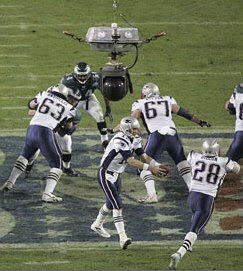
\includegraphics[width=.36\linewidth]{./chapter02/figures/skycam01.jpg}} 
\hfill
    \subfloat[Les c\^ables permettant le contr\^ole du positionnement de la 
cam\'era sont dispos\'es aux quatre coins du stade]{\label{chapter02:fig0view1} 
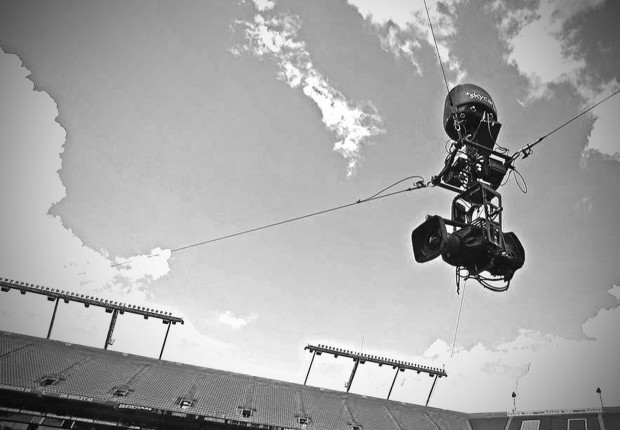
\includegraphics[width=.58\linewidth]{./chapter02/figures/skycam02.jpg}} 
    \caption{\footnotesize{Illustrations de la Skycam}}
\label{chapter02:fig0}
\end{figure}

L'utilisation d'une cam\'era embarqu\'ee sur un manipulateur \`a c\^ables peut 
s'av\'erer pertinente dans un grand nombre de cas : afin d'explorer 
l'environnement dans des op\'erations de sauvetage par exemple, pour d\'etecter 
et suivre des objets sur de longues distances, ou simplement pour rendre le 
contr\^ole robuste aux variations des conditions de manipulation.

Dans le m\^eme temps, nous avons vu que le contr\^ole des robots parall\`eles 
\`a c\^ables pr\'esentait des difficult\'es suppl\'ementaires par rapport aux 
robots parall\`eles classiques et aux robots s\'eries. L'utilisation de 
capteurs int\'eroceptifs et ext\'eroceptifs devrait par exemple permettre de 
corriger des d\'eviations d'estimations (concernant par exemple l'incertitude 
sur la longueur enroul\'ee d'un c\^able sur une poulie) ou des erreurs de 
mod\'elisation (hypoth\`eses sur l'\'elasticit\'e r\'eelle des c\^ables) et 
ainsi am\'eliorer la qualit\'e de contr\^ole. A nouveau, l'ajout d'une ou de 
plusieurs cam\'eras para\^it ici pertinent : on peut ainsi imaginer qu'une 
cam\'era d\'eport\'ee pourrait nous donner la position de l'organe terminal - 
r\'esolvant ainsi le {\it MGD} - ou des mesures sur les articulations 
simplifiant le {\it MGI}. Nous verrons dans la section suivante que ces deux 
strat\'egies ont \'et\'e \'etudi\'ees et fournissent des r\'esultats 
int\'eressants.

Deux questions se posent cependant ici, \`a savoir la lourdeur et la pertinence 
du dispositif de capteurs que nous pouvons utiliser pour am\'eliorer les 
performances d'un manipulateur. Cela d\'epend \'evidemment du contexte de 
l'op\'eration de manipulation : si une cam\'era d\'eport\'ee unique peut 
suffire dans un espace de travail restreint, c'est une solution beaucoup moins 
\'evidente lorsque celui-ci devient v\'eritablement cons\'equent. Lorsque des 
questions d'\'ethique et d'intimit\'e se posent, cela devient m\^eme 
carr\'ement inenvisageable. La multiplication des dispositifs pose quant \`a 
elle la question d'un double co\^ut : co\^ut financier du dispositif, co\^ut en 
temps de calcul du traitement des informations. En particulier, ce dernier est 
\`a comparer au co\^ut des calculs n\'ecessaires au contr\^ole du manipulateur 
sans information suppl\'ementaire pour une performance donn\'ee.

Apr\`es avoir, dans la premi\`ere section de chapitre explor\'e les travaux 
ayant \'et\'e r\'ealis\'es dans le domaine de l'asservissement visuel des 
robots parall\`eles \`a c\^ables, nous indiquerons les raisons pour lesquelles 
nous avons d\'ecid\'e dans ce travail de nous int\'eresser sp\'ecifiquement \`a 
l'utilisation d'une cam\'era embarqu\'ee unique. Dans une seconde section, nous 
pr\'esenterons un sch\'ema d'asservissement simple permettant d'augmenter la 
pr\'ecision et d'am\'eliorer la robustesse d'une op\'eration de manipulation. En 
troisi\`eme section, nous pr\'esenterons un sch\'ema de contr\^ole exploitant 
les informations visuelles pour corriger une commande articulaire. Nous en 
explorerons les avantages et les limites, et d\'eterminerons les conditions de 
son utilisation. La derni\`ere section sera consacr\'ee \`a l'illustration de 
cette loi de commande articulaire.

\section{Travaux pr\'eliminaires}

\subsection{Asservissements en position}

D'abord propos\'e pour le contr\^ole de robots parall\`eles classiques 
\cite{dallej.2006}, l'asservissement visuel en position a par la suite \'et\'e 
adapt\'e aux robots parall\`eles \`a c\^ables afin d'\'eviter l'utilisation de 
capteurs articulaires \cite{dallej2012} \cite{dallej2011}. La m\'ethode 
pr\'esente en particulier deux avantages : d'une part elle devrait \^etre moins 
sensible aux bruits de mesures, et d'autre part le nombre de capteurs utilis\'es 
devrait \^etre moindre.

Au sein de ces travaux, les auteurs proposent tout \`a tour un contr\^ole 
cin\'ematique puis un contr\^ole dynamique. Pour autant -- et bien que la 
question soit mentionn\'ee -- l'impasse est faite sur la gestion de la 
r\'epartiton des tensions dans les diff\'erents c\^ables, et particuli\`erement 
sur l'\'eventuelle absence de tension dans un ou plusieurs c\^ables. C'est en 
effet une limite du seul contr\^ole en position de ne pas \^etre en mesure 
d'indiquer quels sont les c\^ables contr\^olant les d\'eplacements de la 
plate-forme et dans quelle mesure.

Pour le contr\^ole en position, une cam\'era rapide (75Hz) est utilis\'e pour 
d\'etecter et suivre un motif dispos\'e sur l'organe terminal, \`a partir duquel 
les informations visuelles n\'ecessaires \`a l'\'elaboration de la loi de 
commande sont d\'eduites. 


\subsection{Asservissements articulaires}


\section{Sch\'ema classique}

\subsection{Choix de primitives}

\subsection{Cas g\'en\'erique}

\subsection{Cas N-1}


\section{Asservissement visuel dans l'espace articulaire}

\subsection{Formalisation}

\section{Illustrations}

\subsection{${\bf J}_{4 \times 3}$ vs ${\bf J}_{3 \times 3}$}

\subsection{Initialisation}

\subsection{Exemples}


















